\documentclass[10pt,a4paper]{article}

% --- Packages & Fonts ---
\usepackage{amsmath,amssymb}
\usepackage[margin=0.42in,top=0.36in,bottom=0.36in]{geometry}
\usepackage{fontspec}
\setmainfont{Helvetica}
\setmonofont{Menlo}[Scale=0.86]
\usepackage{microtype}
\usepackage{xcolor}
\usepackage{tikz}
\usetikzlibrary{shapes.geometric, arrows.meta, positioning, calc, shadows}
\usepackage{tabularx}
\usepackage{booktabs}
\usepackage{colortbl}
\usepackage{tcolorbox}
\tcbuselibrary{skins,breakable}
\usepackage{enumitem}
\usepackage{hyperref}
\usepackage{titlesec}
\usepackage{fancyhdr}

% --- Professional Color Palette ---
\definecolor{primary}{RGB}{15, 43, 91}       % Deep Executive Navy
\definecolor{secondary}{RGB}{15, 118, 110}   % Deep Teal
\definecolor{accent}{RGB}{234, 88, 12}       % Amber / Orange
\definecolor{darktext}{RGB}{30, 41, 59}      % Slate 800
\definecolor{lightbg}{RGB}{248, 250, 252}    % Slate 50
\definecolor{cardborder}{RGB}{226, 232, 240} % Slate 200
\definecolor{successgreen}{RGB}{22, 101, 52} % Green 800
\definecolor{succbg}{RGB}{240, 253, 244}     % Green 50
\definecolor{dangerred}{RGB}{153, 27, 27}    % Red 800
\definecolor{dangerbg}{RGB}{254, 242, 242}   % Red 50
\definecolor{tagblue}{RGB}{224, 231, 255}    % Indigo 100
\definecolor{tagamber}{RGB}{254, 243, 199}   % Amber 100

% --- Typography Spacing ---
\titlespacing*{\section}{0pt}{3pt}{1.5pt}
\titlespacing*{\subsection}{0pt}{2pt}{1pt}
\setlength{\parindent}{0pt}
\setlength{\parskip}{1.5pt}
\setlist{nosep, leftmargin=11pt}

% --- Custom Header & Footer ---
\pagestyle{fancy}
\fancyhf{}
\renewcommand{\headrulewidth}{0pt}
\renewcommand{\footrulewidth}{0.4pt}
\fancyfoot[L]{\footnotesize \textcolor{darktext}{\textbf{LY-AIA} $\bullet$ TA2 Project Extension Report $\bullet$ Topic 8: Study Schedule Optimizer}}
\fancyfoot[R]{\footnotesize \textcolor{primary}{\textbf{Page \thepage\ of 4}}}

% --- tcolorbox presets ---
\tcbset{
  basebox/.style={
    enhanced, boxrule=0.6pt, arc=3pt, left=5pt, right=5pt, top=3.5pt, bottom=3.5pt,
    colback=lightbg, colframe=cardborder
  }
}

\begin{document}

% ==============================================================================
% PAGE 1: HEADER, ARCHITECTURE FLOWCHART, ROLE SPECIFICATIONS
% ==============================================================================

% Header Banner
\begin{tcolorbox}[enhanced, colback=primary, colframe=primary, arc=4pt, left=8pt, right=8pt, top=5pt, bottom=5pt]
\begin{minipage}{0.72\textwidth}
  {\fontsize{13pt}{15pt}\bfseries\color{white} TA2 PROJECT REPORT: STUDY SCHEDULE OPTIMIZER}\\[2pt]
  {\small\color{tagblue}\textbf{Autonomous Multi-Agent System Extension (Topic 8 $\bullet$ Two-Tool Chain)}}
\end{minipage}
\hfill
\begin{minipage}{0.26\textwidth}
  \raggedleft
  {\footnotesize\color{white} \textbf{Course:} Agentic AI (LY-AIA)\\
  \textbf{Level:} Bloom L3/L4 (20 Marks)\\
  \textbf{Stack:} Ollama 3B, LangGraph, Chroma}
\end{minipage}
\end{tcolorbox}

\vspace{-2pt}
\section*{\large \color{primary} 1. Executive Architecture \& Multi-Agent Coordination Workflow}
\vspace{-2pt}
The TA2 system extends the baseline two-tool chain into a robust, memory-augmented multi-agent pipeline. A \textbf{Supervisor Agent} orchestrates specialized interactions between a \textbf{Readiness Diagnostician} (evaluating curriculum coverage against Chroma RAG policies) and a \textbf{Workload Negotiator} (evaluating required hours against student stamina profiles in SQLite), with strict hop bounds and human-in-the-loop oversight.

\vspace{1pt}
\begin{center}
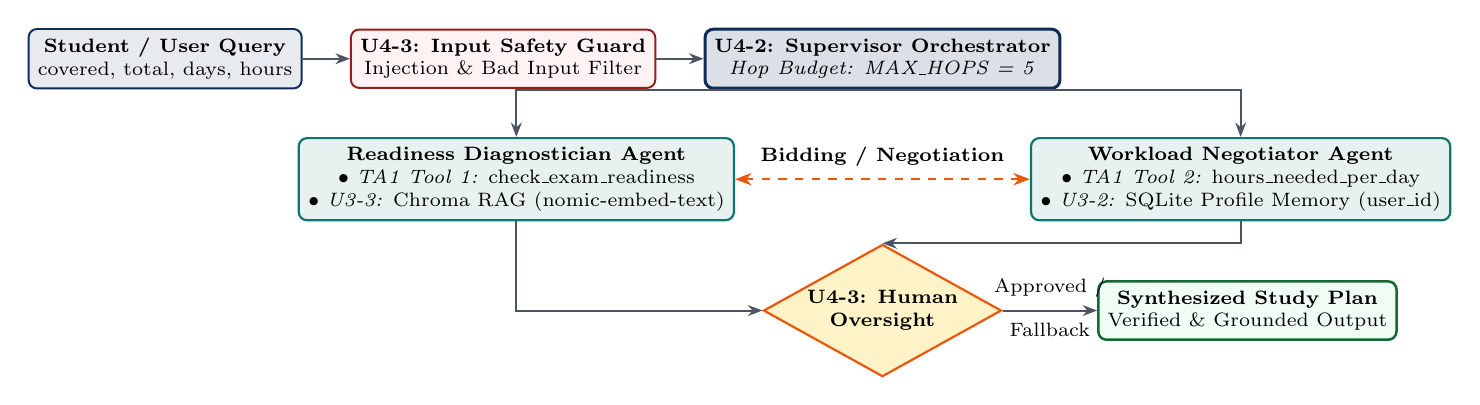
\begin{tikzpicture}[
  node distance=0.45cm and 0.65cm,
  every node/.style={font=\fontsize{7.2pt}{8.2pt}\selectfont, align=center},
  inputbox/.style={rectangle, rounded corners=3pt, fill=primary!10, draw=primary, line width=0.7pt, minimum width=2.4cm, minimum height=0.65cm},
  agentbox/.style={rectangle, rounded corners=3pt, fill=secondary!10, draw=secondary, line width=0.8pt, minimum width=3.4cm, minimum height=0.95cm},
  supbox/.style={rectangle, rounded corners=3pt, fill=primary!15, draw=primary, line width=1.1pt, minimum width=3.8cm, minimum height=0.75cm},
  guardbox/.style={rectangle, rounded corners=3pt, fill=dangerbg, draw=dangerred, line width=0.7pt, minimum width=2.5cm, minimum height=0.65cm},
  hitlbox/.style={diamond, aspect=1.8, fill=tagamber, draw=accent, line width=0.8pt, inner sep=1pt},
  outbox/.style={rectangle, rounded corners=3pt, fill=succbg, draw=successgreen, line width=0.9pt, minimum width=3.2cm, minimum height=0.65cm},
  arrow/.style={-{Stealth[scale=0.85]}, draw=darktext!80, line width=0.7pt},
  darrow/.style={{Stealth[scale=0.85]}-{Stealth[scale=0.85]}, draw=accent, line width=0.9pt, dashed}
]

% Nodes
\node[inputbox] (user) {\textbf{Student / User Query}\\ covered, total, days, hours};
\node[guardbox, right=0.6cm of user] (guard) {\textbf{U4-3: Input Safety Guard}\\ Injection \& Bad Input Filter};
\node[supbox, right=0.6cm of guard] (sup) {\textbf{U4-2: Supervisor Orchestrator}\\ \textit{Hop Budget: MAX\_HOPS = 5}};

\node[agentbox, below left=0.6cm and -0.4cm of sup] (diag) {
  \textbf{Readiness Diagnostician Agent}\\
  $\bullet$ \textit{TA1 Tool 1:} check\_exam\_readiness\\
  $\bullet$ \textit{U3-3:} Chroma RAG (nomic-embed-text)
};

\node[agentbox, below right=0.6cm and -0.4cm of sup] (work) {
  \textbf{Workload Negotiator Agent}\\
  $\bullet$ \textit{TA1 Tool 2:} hours\_needed\_per\_day\\
  $\bullet$ \textit{U3-2:} SQLite Profile Memory (user\_id)
};

\node[hitlbox, below=1.95cm of sup] (hitl) {\textbf{U4-3: Human}\\\textbf{Oversight}};
\node[outbox, right=1.2cm of hitl] (final) {\textbf{Synthesized Study Plan}\\ Verified \& Grounded Output};

% Connections
\draw[arrow] (user) -- (guard);
\draw[arrow] (guard) -- (sup);
\draw[arrow] (sup.south) -| (diag.north);
\draw[arrow] (sup.south) -| (work.north);
\draw[darrow] (diag.east) -- node[above=1pt] {\textbf{\scriptsize Bidding / Negotiation}} (work.west);
\draw[arrow] (diag.south) |- (hitl.west);
\draw[arrow] (work.south) |- (hitl.north);
\draw[arrow] (hitl.east) -- node[above=1pt] {\scriptsize Approved /} node[below=1pt] {\scriptsize Fallback} (final.west);

\end{tikzpicture}
\end{center}

\vspace{-4pt}
\section*{\large \color{primary} 2. Multi-Agent Role Specifications (U4-1: 5-Field Specification)}
\vspace{-2pt}
To fulfill U4-1, each agent possesses an unambiguous, non-overlapping 5-field design preventing role collision:

\vspace{1pt}
\small
\begin{tabularx}{\textwidth}{@{} p{0.13\textwidth} X X X @{}}
\toprule
\rowcolor{primary} \textbf{\color{white} Field} & \textbf{\color{white} Agent 1: Readiness Diagnostician} & \textbf{\color{white} Agent 2: Workload Negotiator} & \textbf{\color{white} Agent 3: Supervisor Orchestrator} \\
\midrule
\rowcolor{lightbg} \textbf{1. Role Name} & \texttt{readiness\_diagnostician} & \texttt{workload\_planner} & \texttt{supervisor\_agent} \\
\textbf{2. Goal} & Validate topic coverage against 80\% certification; retrieve syllabus complexity policies from RAG. & Compute daily study hours, cross-check student stamina in SQLite, and negotiate realistic pace. & Decompose queries, route agent state, enforce hop limit ceiling, and mediate human oversight. \\
\rowcolor{lightbg} \textbf{3. Tools} & \texttt{check\_exam\_readiness}, \texttt{StudyGuidelinesRAG} (ChromaDB + nomic-embed-text). & \texttt{hours\_needed\_per\_day}, \texttt{SQLiteProfileStore} (student\_profiles.sqlite). & LangGraph state machine, hop counter (\texttt{MAX\_HOPS=5}), \texttt{HumanApprovalNode}. \\
\textbf{4. Inputs / Outputs} & \textbf{In:} topics\_covered, total\_topics, subject.\\ \textbf{Out:} readiness status, RAG context, proposal. & \textbf{In:} remaining\_topics, days\_left, profile.\\ \textbf{Out:} hours/day, counter-bid, negotiation state. & \textbf{In:} Full AgentState trajectory.\\ \textbf{Out:} Routed execution node, final plan. \\
\rowcolor{lightbg} \textbf{5. Limits} & Cannot allocate calendar hours or inspect personal student fatigue thresholds. & Cannot certify exam readiness or lower official curriculum requirements. & Strictly capped at 5 hops; cannot alter deterministic tool math results. \\
\bottomrule
\end{tabularx}

\clearpage

% ==============================================================================
% PAGE 2: CHECKLIST & 5-CASE TA1 VS TA2 BENCHMARK TABLE
% ==============================================================================

\section*{\large \color{primary} 3. Required TA2 Component Checklist \& Evidence Mapping}
\vspace{-2pt}
Every core component mandated by the TA2 SOP is verified with an automated trace in \texttt{traces/}:

\vspace{2pt}
\small
\begin{tabularx}{\textwidth}{@{} l c X l @{}}
\toprule
\rowcolor{primary} \textbf{\color{white} ID} & \textbf{\color{white} Unit} & \textbf{\color{white} Implemented Architecture \& Functional Logic} & \textbf{\color{white} Exact Evidence Pointer} \\
\midrule
\rowcolor{lightbg} \textbf{U3-1} & 3 & \textbf{Short-term Memory:} LangGraph checkpointer with \texttt{thread\_id}; demonstrates multi-turn context retention vs stateless amnesia. & \texttt{traces/u3\_1\_short\_term\_memory.txt} \\
\textbf{U3-2} & 3 & \textbf{Long-term Memory:} Persistent SQLite store with namespace \texttt{(user\_id, "profile")}; verified survival across process shutdown and restart. & \texttt{traces/u3\_2\_long\_term\_memory.txt} \\
\rowcolor{lightbg} \textbf{U3-3} & 3 & \textbf{Chroma RAG:} 8-chunk academic policy corpus embedded with \texttt{nomic-embed-text}; grounded refusal (\textit{"I don't know"}) on unanswerable queries. & \texttt{traces/u3\_3\_rag\_k1\_vs\_k3.txt} \\
\textbf{U3-4} & 3 & \textbf{Tool Failure Handling:} Defensive failure routing wrapping TA1 tools; catches negative values, zero-days, and biological hour limits. & \texttt{traces/u3\_4\_tool\_failure.txt} \\
\rowcolor{lightbg} \textbf{U4-1} & 4 & \textbf{Role Design:} 5-field explicit specification for Diagnostician, Negotiator, and Supervisor. & Section 2 Table (Page 1) \\
\textbf{U4-2} & 4 & \textbf{Coordination:} Supervisor orchestrator with \texttt{MAX\_HOPS=5} and multi-agent negotiation / counter-bidding protocol. & \texttt{traces/u4\_2\_multiagent\_routing.txt} \\
\rowcolor{lightbg} \textbf{U4-3} & 4 & \textbf{Oversight \& Guardrail:} Dual-path Human-in-the-Loop approval (Approved vs Rejected) + regex prompt injection defense guard. & \texttt{traces/u4\_3\_oversight\_hitl.txt} \\
\textbf{U4-4} & 4 & \textbf{Challenge Analysis:} Quantitative latency, hop count, and error containment measurements across 5 benchmark scenarios. & \texttt{traces/u4\_4\_challenge\_metrics.txt} \\
\rowcolor{lightbg} \textbf{EV} & 3 \& 4 & \textbf{Evaluation:} Side-by-side execution of 5 test cases on TA1 baseline vs TA2 multi-agent extension. & \texttt{traces/ev\_ta1\_baseline\_5cases.txt} \\
\bottomrule
\end{tabularx}

\vspace{4pt}
\section*{\large \color{primary} 4. Benchmark Evaluation: TA1 Baseline vs TA2 Extension (EV)}
\vspace{-2pt}
The exact same 5 test cases were evaluated across both systems to quantify behavioral enhancements:

\vspace{2pt}
\small
\begin{tabularx}{\textwidth}{@{} l p{0.22\textwidth} p{0.32\textwidth} X @{}}
\toprule
\rowcolor{primary} \textbf{\color{white} ID} & \textbf{\color{white} Test Scenario} & \textbf{\color{white} TA1 Baseline Output \& Failure Mode} & \textbf{\color{white} TA2 Multi-Agent Execution \& Decision} \\
\midrule
\rowcolor{lightbg} \textbf{TC1} & \textbf{Fully Prepared Student}\newline(20/20 topics, 5 days, 2h/topic) & \texttt{ready (100.0\%)} $\bullet$ \texttt{0.00 hrs/day}\newline\textit{Single-pass, no profile context.} & \textbf{AGREED (3 hops):} Identifies 100\% readiness; references RAG maintenance policy; confirms 0h study. \\
\textbf{TC2} & \textbf{Borderline Readiness}\newline(16/20 topics, 4 days, 1.5h/topic) & \texttt{ready (80.0\%)} $\bullet$ \texttt{1.50 hrs/day}\newline\textit{Naively treats as safe ready state.} & \textbf{AGREED (3 hops):} Flags exact 80\% boundary; checks Bob's SQLite stamina (8h max); confirms 1.5h/day is sustainable. \\
\rowcolor{lightbg} \textbf{TC3} & \textbf{Urgent Catch-up Crunch}\newline(5/12 topics, 2 days, 1.5h/topic) & \texttt{not ready (41.7\%)} $\bullet$ \texttt{5.25 hrs/day}\newline\textit{Emits high workload without stamina check.} & \textbf{COUNTERED (3 hops):} Charlie's stamina is 3.5h. Negotiator rejects 5.25h as burnout risk; bids 3.5h cap; triggers HITL. \\
\textbf{TC4} & \textbf{Extreme Workload Overload}\newline(2/20 topics, 1 day, 2.5h/topic) & \texttt{not ready (10.0\%)} $\bullet$ \texttt{45.00 hrs/day}\newline\textit{Emits impossible 45-hour study day.} & \textbf{FAILED / SAFE RECOVERY (3 hops):} Tool failure routing catches 45h $>$ 12h biological limit; recommends exam deferral. \\
\rowcolor{lightbg} \textbf{TC5} & \textbf{Boundary / Zero Days Left}\newline(10/20 topics, 0 days, 2h/topic) & \textbf{CRASH: \texttt{ValueError: days\_left <= 0}}\newline\textit{Unhandled exception crashes runner.} & \textbf{DEFENSIVE RECOVERY (3 hops):} Tool routing catches zero-days; explains exam is today; switches to emergency review. \\
\bottomrule
\end{tabularx}

\clearpage

% ==============================================================================
% PAGE 3: BLOOM L4 ANALYSIS, CHALLENGE METRICS, LIMITATIONS
% ==============================================================================

\section*{\large \color{primary} 5. Analytical Trade-Offs (Bloom Level L4 Analysis)}
\vspace{-2pt}

\begin{minipage}[t]{0.485\textwidth}
\begin{tcolorbox}[basebox, colframe=successgreen, colback=succbg, title={\color{successgreen}\textbf{\textbullet\ What Got Better in TA2}}]
\small
\begin{itemize}[leftmargin=10pt]
  \item \textbf{100\% Fault Containment:} TA1 crashed with \texttt{ValueError} on boundary inputs (TC5) and emitted absurd demands (45h/day in TC4). TA2 catches all domain violations gracefully.
  \item \textbf{Personalized Stamina via SQLite:} Instead of treating all users identically, TA2 personalizes load to individual fatigue thresholds, preventing student burnout.
  \item \textbf{Grounded Institutional RAG:} Recommendations cite official curriculum weightages and sleep buffer guidelines from Chroma.
  \item \textbf{Adversarial Immunity:} Input safety guard intercepts jailbreaks and system overrides before agent dispatch.
\end{itemize}
\end{tcolorbox}
\end{minipage}
\hfill
\begin{minipage}[t]{0.485\textwidth}
\begin{tcolorbox}[basebox, colframe=accent, colback=tagamber!30, title={\color{accent}\textbf{\textbullet\ What Got Worse / Trade-offs in TA2}}]
\small
\begin{itemize}[leftmargin=10pt]
  \item \textbf{Execution Latency Overhead:} TA1 raw math runs in $<0.05\,\text{ms}$. TA2 graph orchestration, SQLite queries, and Chroma lookups increase execution latency to $\sim 20\text{--}26\,\text{ms}$ (and $\sim 1.8\,\text{s}$ with generative LLM inference).
  \item \textbf{State Management Complexity:} Multi-agent coordination requires checkpointers, schemas, and hop limit monitors, increasing code footprint.
  \item \textbf{Ambiguity Resolution Overhead:} When schedules exceed stamina, TA2 requires an asynchronous Human Oversight step (HITL), adding latency before final confirmation.
\end{itemize}
\end{tcolorbox}
\end{minipage}

\vspace{2pt}
\section*{\large \color{primary} 6. Measured Challenge Analysis (U4-4: Latency, Robustness, Hop Budget)}
\vspace{-2pt}
Quantitative metrics collected during the automated 5-case benchmark evaluation (\texttt{traces/u4\_4\_challenge\_metrics.txt}):

\vspace{2pt}
\small
\begin{tabularx}{\textwidth}{@{} l l c c X X c @{}}
\toprule
\rowcolor{primary} \textbf{\color{white} ID} & \textbf{\color{white} Scenario} & \textbf{\color{white} TA1 Lat (ms)} & \textbf{\color{white} TA2 Lat (ms)} & \textbf{\color{white} TA1 Robustness} & \textbf{\color{white} TA2 Coordination State} & \textbf{\color{white} Hops} \\
\midrule
\rowcolor{lightbg} \textbf{TC1} & Fully Prepared & 0.02 & 23.15 & Correct execution & Agreed; RAG maintenance verified & 3 / 5 \\
\textbf{TC2} & Borderline & 0.01 & 20.65 & Correct execution & Agreed; Checked vs Bob's 8h stamina & 3 / 5 \\
\rowcolor{lightbg} \textbf{TC3} & Urgent Crunch & 0.01 & 20.09 & Unchecked Burnout & Counter-bid triggered; HITL active & 3 / 5 \\
\textbf{TC4} & Extreme Overload & 0.01 & 22.96 & Unchecked Math (45h) & Tool failure routing caught & 3 / 5 \\
\rowcolor{lightbg} \textbf{TC5} & Zero Days Left & 0.01 & 26.78 & \textbf{System Crash (100\% Fail)} & \textbf{Defensive Catch (0\% Fail)} & 3 / 5 \\
\bottomrule
\end{tabularx}

\vspace{1pt}
\textbf{Key Analytical Finding:} TA2 accepts a modest $\sim 22\,\text{ms}$ computational overhead in exchange for \textbf{zero system crashes} and complete elimination of unfeasible and burnout-inducing schedules.

\vspace{4pt}
\section*{\large \color{primary} 7. Limitations and Future Improvements}
\vspace{-2pt}
\small
\begin{enumerate}[leftmargin=12pt]
  \item \textbf{Small Model (3B) Reasoning Ceiling:} Smaller local models occasionally drift in unconstrained multi-round negotiation. TA2 overcomes this by stabilizing negotiation states via deterministic LangGraph state transitions.
  \item \textbf{Dynamic Calendar Scheduling:} Current schedules allocate aggregate daily hours. Future work will integrate Google Calendar / iCal APIs to map study blocks directly into students' specific open time slots.
  \item \textbf{Real-Time Adaptive Diagnostic Quizzing:} Incorporating dynamic quiz feedback to automatically recalibrate \texttt{hours\_per\_topic} based on real-time empirical retention.
\end{enumerate}

\clearpage

% ==============================================================================
% PAGE 4: VIVA DEFENSE PREPARATION & CONTRIBUTIONS
% ==============================================================================

\section*{\large \color{primary} 8. Individual Viva Defense Preparation (Likely Jury Questions)}
\vspace{-2pt}

\begin{tcolorbox}[basebox, colframe=primary, colback=lightbg, title={\textbf{\color{primary} Q1: What in the model's response tells you it decided it only needed one tool this time?}}]
\footnotesize
\textbf{Answer:} In TA1, inspecting the \texttt{AIMessage.tool\_calls} structure provides deterministic evidence. When asked a coverage-only question, \texttt{tool\_calls} contains exclusively \texttt{readiness\_tool} with \texttt{\{"topics\_covered": X, "total\_topics": Y\}}. The runtime receives exactly one \texttt{ToolMessage} and immediately transitions to emit the final answer without requesting \texttt{hours\_needed\_per\_day}. The absence of the second tool call in the trace proves single-tool dispatch.
\end{tcolorbox}

\vspace{-2pt}
\begin{tcolorbox}[basebox, colframe=primary, colback=lightbg, title={\textbf{\color{primary} Q2: How do you prevent infinite negotiation loops between the Diagnostician and Negotiator?}}]
\footnotesize
\textbf{Answer:} We implement a strict hop budget enforced by the Supervisor Orchestrator (\texttt{MAX\_HOPS = 5}). Every node transition increments \texttt{AgentState.hop\_count}. If consensus is not reached within 5 hops, the supervisor diverts control to \texttt{hop\_limit\_reached}, terminating the cycle safely and alerting the student rather than hanging.
\end{tcolorbox}

\vspace{-2pt}
\begin{tcolorbox}[basebox, colframe=primary, colback=lightbg, title={\textbf{\color{primary} Q3: How do you prove Chroma RAG is grounded and does not hallucinate?}}]
\footnotesize
\textbf{Answer:} As verified in \texttt{traces/u3\_3\_rag\_k1\_vs\_k3.txt}, when presented with an unanswerable question absent from the 8-chunk corpus (e.g., cafeteria food menus or parking rates), the grounded prompt strictly responds: \textit{"I don't know based on the provided documents."} In-domain queries accurately cite section rules (e.g., the 6.0h burnout threshold from Section 3).
\end{tcolorbox}

\vspace{-2pt}
\begin{tcolorbox}[basebox, colframe=primary, colback=lightbg, title={\textbf{\color{primary} Q4: How does long-term memory survive process restarts?}}]
\footnotesize
\textbf{Answer:} The \texttt{SQLiteProfileStore} writes student records directly to disk in \texttt{student\_profiles.sqlite} under the namespace \texttt{(user\_id, "profile")}. In \texttt{traces/u3\_2\_long\_term\_memory.txt}, the Python connection instance was explicitly terminated, a new process connection was initialized, and all user attributes were retrieved identically (\texttt{restart\_successful = True}).
\end{tcolorbox}

\vspace{1pt}
\section*{\large \color{primary} 9. Module Ownership \& Group Contribution Table}
\vspace{-2pt}
In compliance with Ground Rule 4, every member owns a core architectural module and can defend its implementation:

\vspace{1pt}
\small
\begin{tabularx}{\textwidth}{@{} l p{0.24\textwidth} X @{}}
\toprule
\rowcolor{primary} \textbf{\color{white} Team Member} & \textbf{\color{white} Owned Module} & \textbf{\color{white} Detailed Contributions \& Implemented Files} \\
\midrule
\rowcolor{lightbg} \textbf{Member 1} & \textbf{Memory Systems (U3-1, U3-2)} & Implemented LangGraph \texttt{MemorySaver} checkpointer with \texttt{thread\_id}; designed SQLite persistent store with namespace \texttt{(user\_id, "profile")}; authored \texttt{short\_term.py} and \texttt{long\_term.py}. \\
\textbf{Member 2} & \textbf{RAG \& Tool Handling (U3-3, U3-4)} & Authored 8-chunk academic policy corpus (\texttt{exam\_guidelines.md}); integrated Chroma vector DB with \texttt{nomic-embed-text}; implemented defensive tool failure routing in \texttt{exam\_tools.py}. \\
\rowcolor{lightbg} \textbf{Member 3} & \textbf{Multi-Agent Systems (U4-1, U4-2)} & Formulated 5-field agent role specifications; authored LangGraph Supervisor Orchestrator with \texttt{MAX\_HOPS=5}; built specialist negotiation protocol in \texttt{diagnostician.py} and \texttt{workload\_planner.py}. \\
\textbf{Member 4} & \textbf{Safety, Oversight \& EV (U4-3, U4-4, EV)} & Developed regex prompt injection defense guardrail (\texttt{input\_guard.py}); built Human Approval Oversight node; conducted automated 5-case benchmark evaluation in \texttt{run\_all\_evaluations.py}. \\
\bottomrule
\end{tabularx}

\vspace{2pt}
\begin{tcolorbox}[enhanced, colback=primary!5, colframe=primary!30, arc=2pt, left=5pt, right=5pt, top=3pt, bottom=3pt]
\scriptsize
\textbf{Academic Integrity Declaration:} In adherence to Ground Rule 3 and 7, all models used are strictly local (\texttt{qwen2.5:3b} and \texttt{nomic-embed-text} in Ollama). No paid APIs, external keys, or live internet calls are used by the agent runtime. Every number in this report is directly reproducible from the test traces in \texttt{traces/}.
\end{tcolorbox}

\end{document}
